\documentclass[10pt]{article}

\usepackage{lipsum}
\usepackage{url}
\usepackage{float}
\usepackage{amsmath}
\usepackage{enumitem}
\usepackage{graphicx}
\usepackage{caption}
\usepackage{subcaption}
\usepackage{rotating}
\usepackage{geometry}
\usepackage{listings}
\usepackage{hyperref}
\usepackage[T1]{fontenc}
\usepackage[numbered]{matlab-prettifier}

\newcommand{\documentTitle}{Lab 7 - Digital Logic}
\newcommand{\documentAuthor}{Andrew Pham, Aneel Damaraju}
\newcommand{\courseTitle}{ELEC 240}
\newcommand{\testDate}{October 23, 2018}
\newcommand{\reportDate}{November 2, 2018}

\geometry{margin=1in}
\lstset{
    tabsize=4,
    basicstyle={\ttfamily},
    captionpos=b,
    belowskip=1em,
    aboveskip=1em,
    numbers=left,
	escapechar=\@,
}

\title{
    \textbf{\courseTitle} \\
    \textbf{\documentTitle} \\
    \bigskip
    \textbf{\large{Test performed: \testDate}} \\
    \textbf{\large{Report submitted: \reportDate}} \\
    \bigskip
    \bigskip
}
\author{\documentAuthor}
\date{}

\begin{document}

\maketitle

\newpage

\section{Objective}

The objective of this lab was to learn the underlying logical operations behind an adder and to then apply these principles to implement a one-bit full adder on a breadboard. 

\medskip

%\textit{Note (To be deleted): Think of this test report as a document with your peers as your readers. This means you can assume a similar knowledge background as you. Your readers should be able to easily understand what is going on, and also be able to repeat your lab results based on your document and all references you cite.}

%\textit{For the Objective section, identify the test you performed and its objectives. The objectives of the test are important to state because they are usually analyzed in the conclusion to determine whether the test succeeded.}

\section{Materials}

\begin{itemize}
	\item Test Board
	\item 1x 74HC00 Quad 2-input NAND gate
	\item 1x 7486 Quad 2-input XOR gate
	\item 2x LEDs
	\item 1x Quad DIP switch
	\item 5x 330$\Omega$ resistors
	\item Yellow, Red, and Black wire (signal, power, gnd)
	\item Wire strippers and cutters
\end{itemize}

\medskip

%\textit{Note (To be deleted): Provide a bullet point list of components, software tools, and hardware (such as the NI VirtualBench or DMM) used during the lab}

\section{Test Description}

In the first section of the lab, we learned about the logic underlying the fundamental NAND and XOR gates and their truth tables for all combinations of inputs. We then formulated an expression for the correct output of the adder for the three input bits. We then applied DeMorgan's law to simplify the circuit so that it only uses NAND and XOR gates, and we then constructed the one-bit full adder. 

\medskip

%\textit{Note (To be deleted): This section provides a summary of the test your team performed. Give enough information so readers can understand what you did, but do not go into the details of every step.}

\subsection{Pre-Lab Calculations and Schematics}
To begin, we had to understand the underlying logic behind a NAND and a XOR gate, which the adder was composed of. Below in Figure \ref{NAND} is the truth table for a NAND gate, and in Figure \ref{XOR} is the truth table for a XOR gate. 

\begin{figure} [H]
	\begin{table}[H]
		\centering
		\begin{tabular}{||c c c||} 
			\hline
			A & B &  A NAND B\\ [0.5ex] 
			\hline\hline
			0 & 0 & 1\\ 
			0 & 1 & 1\\
			1 & 0 & 1\\
			1 & 1 & 0\\ [1ex] 
			\hline
		\end{tabular}
	\end{table}
	\caption{NAND Truth Table}
	\label{NAND}
\end{figure}

\begin{figure} [H]
	\begin{table}[H]
		\centering
		\begin{tabular}{||c c c||} 
			\hline
			A & B &  A NAND B\\ [0.5ex] 
			\hline\hline
			0 & 0 & 0\\ 
			0 & 1 & 1\\
			1 & 0 & 1\\
			1 & 1 & 0\\ [1ex] 
			\hline
		\end{tabular}
	\end{table}
	\caption{XOR Truth Table}
	\label{XOR}
\end{figure}

We then derived the following expression for the Sum $S$ and Carry $C$ output bits of the adder based on the three one-bit inputs $x,y,z$. 

$$ S = (x \bigoplus y) \bigoplus z$$
$$ C = (x \bullet y) \vee (x \bigoplus y) \bullet z $$

We then created the following truth table for the sum and carry bits based on these outputs as follows in Fig \ref{sum}:

\begin{figure} [H]
	\begin{table}[H]
		\centering
		\begin{tabular}{||c c c c c c c c c||} 
			\hline
			x & y &  z & $x \bullet y$ & $x \bigoplus y$ & $(x \bigoplus y) \bigoplus z$ & $ (x \bullet y) \vee (x \bigoplus y) $ & C & S\\ [0.5ex] 
			\hline\hline
			0 & 0 & 0 & 0 & 0 & 0 & 0 & 0 & 0\\ 
			0 & 0 & 1 & 0 & 0 & 1 & 0 & 0 & 1\\
			0 & 1 & 0 & 0 & 1 & 1 & 1 & 0 & 1\\
			0 & 1 & 1 & 0 & 1 & 0 & 1 & 1 & 0\\
			1 & 0 & 0 & 0 & 1 & 1 & 1 & 0 & 1\\
			1 & 0 & 1 & 0 & 1 & 0 & 1 & 1 & 0\\
			1 & 1 & 0 & 0 & 0 & 1 & 0 & 0 & 1\\
			1 & 1 & 1 & 1 & 0 & 1 & 1 & 1 & 1\\[1ex] 
			\hline
		\end{tabular}
	\end{table}
	\caption{Naive Truth Table for the Sum and Carry bits}
	\label{sum}
\end{figure}

However, the direct implementation of the above truth table into logic requires the use of 2 XOR gates for the sum bit 2 NAND gates, and 1 OR gate for the carry bit. Since we want to reduce the complexity of our adder, we can use DeMorgan's laws to simplify the requirements for the carry bits:

$$ x \bullet y = \lnot (x \vee y) $$
$$ x \vee y = \lnot (x \bullet y) $$

We then obtain the following equation for the carry bit expression by applying the above DeMorgan's laws:

$$ C = \lnot 
\left( 
\lnot (x \bullet y) \bullet \lnot 
\left( 
\left(x \bigoplus y \right) \bullet z 
\right) 
\right) $$

The truth table is depicted below in Fig \ref{mod};

\begin{figure} [H]
	\begin{table}[H]
		\centering
		\begin{tabular}{||c c c c c c c c||} 
			\hline
			x & y &  z & $x \bullet y$ & $x \bigoplus y$ & $\lnot ((x \bigoplus y) \bullet z)$ & $ \lnot(x \bullet y) \bullet \lnot ((x \bigoplus y) \bullet z)$ & C\\ [0.5ex] 
			\hline\hline
			0 & 0 & 0 & 0 & 0 & 1 & 1 & 0\\ 
			0 & 0 & 1 & 0 & 0 & 1 & 1 & 0\\
			0 & 1 & 0 & 0 & 1 & 1 & 1 & 0\\
			0 & 1 & 1 & 0 & 1 & 0 & 0 & 1\\
			1 & 0 & 0 & 0 & 1 & 1 & 1 & 0\\
			1 & 0 & 1 & 0 & 1 & 0 & 0 & 1\\
			1 & 1 & 0 & 0 & 0 & 1 & 1 & 0\\
			1 & 1 & 1 & 1 & 0 & 1 & 0 & 1\\[1ex] 
			\hline
		\end{tabular}
	\end{table}
	\caption{Modified Truth Table for the Sum and Carry bits}
	\label{mod}
\end{figure}

The circuit that implements this truth table's equation is depicted below in Fig \ref{fig:circuit} :

\begin{centering}
	\begin{figure} [H]
		\centering
		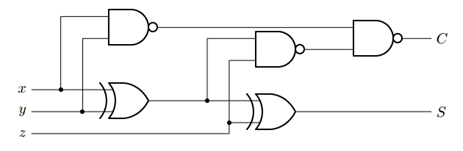
\includegraphics[scale=0.75]{images/fulladder_2.png}
		\caption{One-Bit Full Adder Circuit Diagram}
		\label{fig:circuit}
	\end{figure}
\end{centering}

\medskip

%\textit{Note (To be deleted): Include the homework pre-calculations and schematics that serve as the initial setup for the test. Briefly explain the importance of each item you include. You may want to number your equations/figures so you can refer to them in later sections. Including photos of handwritten work is okay.}

\section{Results and Discussion}

Your text here

\medskip

\textit{Note (To be deleted): The heart of your report is the presentation of your results and a discussion of those results. In your discussion, you should not only analyze your results, but also discuss the implications of those results.}

\section{References}

Your text here

\medskip

\textit{Note (To be deleted): List any datasheets, websites, lab procedure, etc. used during the lab.}

\section{Conclusion}

Your text here

\medskip

\textit{Note (To be deleted): While the ``Results and Discussion'' section focused on the test results individually, the ``Conclusion'' discusses the results in the context of the entire experiment. Usually, the objectives given in the ``Introduction'' are reviewed to determine whether the experiment succeeded. If the objectives were not met, you should analyze why the results were not as predicted.}

\section{Errors}

Your text here

\medskip

\textit{Note (To be deleted): Briefly list sources of error and discuss how to eliminate or deal with them}

\end{document}
